% ============================================================================
%  ПОСТЕР: Результаты методических работ по изучению характеристик
%  стенда проведения нейтронной активации
%  Класс: baposter (A0, portrait)
% ============================================================================
\documentclass[
portrait,
% landscape,
a0paper%,
%draft
]
{baposter}

% ==================== РУСИФИКАЦИЯ ====================
\usepackage{fontspec}
\usepackage[sfdefault]{ClearSans}       % Основной шрифт (гротеск)

% ==================== НАСТРОЙКИ ЯЗЫКА ====================
\usepackage{polyglossia}
\setdefaultlanguage{russian}
\setotherlanguage{english}

% КЛЮЧЕВОЕ: определяем шрифты для кириллицы
\newfontfamily{\cyrillicfont}{ClearSans}
\newfontfamily{\cyrillicfonttt}{Courier New}

% ==================== ПОДАВЛЕНИЕ ПРЕДУПРЕЖДЕНИЙ ====================
\usepackage{silence}
\WarningFilter{fontspec}{Missing character}
\WarningFilter{*}{Missing character}
\WarningFilter{pgf}{Snakes have been superseded}

% ==================== СТАНДАРТНЫЕ ПАКЕТЫ ====================
\usepackage{graphicx}                      % Для вставки картинок
\usepackage[percent]{overpic}              % Для подписей поверх изображений
\usepackage[detect-weight]{siunitx}        % Для физических единиц
\sisetup{
    output-decimal-marker={,},             % Запятая как десятичный разделитель
    group-separator={.},                   % Точка как разделитель тысяч
}
\usepackage{tabto}                         % Для табуляции
\usepackage{booktabs}                      % Для красивых таблиц
\usepackage{amsmath}                       % Математические формулы
\usepackage{float}                         % Управление плавающими объектами
\usepackage{multirow}                      % Объединение строк в таблицах
\usepackage{url}                           % Для форматирования URL
\usepackage{enumitem}                      % Для настройки списков
\usepackage{qrcode}                        % Для генерации QR-кодов
\usepackage{xcolor}                        % Для работы с цветами
\usepackage{ulem}                          % Для подчеркивания
\usepackage{caption}                       % Для подписей рисунков

% ==================== РАЗМЕРЫ ШРИФТОВ (единая точка настройки) ====================
% Формат \fontsize{X}{Y}\selectfont:
%   X — кегль, Y — межстрочный интервал (обычно X*1.2).

% --- Заголовок постера (две строки в шапке) ---
\newcommand{\PosterTitleSize}{\fontsize{15}{17}\selectfont}

% --- Авторы в шапке ---
\newcommand{\PosterAuthorsSize}{\fontsize{9}{11}\selectfont}

% --- Аффилиации в шапке ---
\newcommand{\PosterAffilSize}{\fontsize{8}{10}\selectfont}

% --- Заголовки блоков (\headerbox) ---
\newcommand{\BoxHeaderSize}{\fontsize{11}{13}\selectfont}

% --- Основной текст блоков ---
\newcommand{\BoxBodySize}{\fontsize{8}{9.2}\selectfont}

% --- Подписи под рисунками (captionof) ---
\newcommand{\FigCaptionFont}{\scriptsize}     % можно \small, \footnotesize и т.п.

% --- Подписи в нижнем колонтитуле: ФИО/контакты ---
\newcommand{\FooterContactSize}{\fontsize{8}{9}\selectfont}

% --- Заголовок «ОСНОВНЫЕ ИСТОЧНИКИ» ---
\newcommand{\FooterBibHeadSize}{\fontsize{8}{9}\selectfont}

% --- Сама библиография ---
\newcommand{\FooterBibSize}{\fontsize{7}{8}\selectfont}

% --- Применение подписей (caption) ---
\DeclareCaptionFont{FigCaptionFont}{\FigCaptionFont}
\captionsetup[figure]{font=FigCaptionFont, skip=2pt}

% ==================== НАСТРОЙКИ BIBLATEX ====================
\usepackage[backend=biber,
            style=gost-numeric,            % ГОСТ стиль для русских источников
            sorting=none,                  % Сортировка по порядку цитирования
            language=auto,
            autolang=other,
            maxnames=1,
            minnames=1]{biblatex}
\addbibresource{poster.bib}             % Файл с библиографией

\renewcommand*{\bibfont}{\FooterBibSize}

\usepackage{letltxmacro}

% Сохраняем исходное \emph (подчеркивание от ulem)
\LetLtxMacro{\underlinemph}{\emph}

% Определяем команду для курсивного выделения
\newcommand{\italicemph}[1]{\textit{#1}}

% Внутри библиографии используем курсив
\AtBeginBibliography{%
    \let\emph\italicemph
}

% СОКРАЩЁННЫЙ ФОРМАТ БИБЛИОГРАФИИ
\AtEveryBibitem{%
    \clearfield{title}%
    \clearfield{subtitle}%
    \clearfield{doi}%
    \clearfield{issn}%
    \clearfield{isbn}%
    \clearfield{note}%
    \clearfield{abstract}%
    \clearfield{urldate}%
    \clearlist{url}%
    \clearfield{language}%
}

% ==================== НАСТРОЙКИ ====================
\newlength{\mytextsize}
\newcommand\e{\cdot 10^}                   % Сокращение для научной нотации
\setlength{\unitlength}{1.0cm}             % ВАЖНО: 1 единица picture = 1 см

% ==================== ЦВЕТОВАЯ ПАЛИТРА NSMD ====================
% База — приглушённый синий (чуть темнее) #2E5585
\definecolor{cernblue}{RGB}{46,85,133}      % алиас (совпадает с NSMD)
\definecolor{NSMD}{RGB}{46,85,133}          % основной синий #2E5585
\definecolor{NSMDDark}{RGB}{27,52,84}       % затемнённый (для контраста)
\definecolor{NSMDMid}{RGB}{74,110,160}      % средний оттенок
\definecolor{NSMDLight}{RGB}{205,217,232}   % светлый (фон/подложки)
\definecolor{NSMDPale}{RGB}{236,241,247}    % почти белый с синевой
\definecolor{NSMDAccent}{RGB}{86,120,170}   % акцент для ссылок

% Настройка списков (компактные отступы)
\setlist{noitemsep, topsep=0pt, parsep=0pt, partopsep=0pt, leftmargin=10pt}

% Настройка компактной библиографии
\setlength{\bibitemsep}{0pt}
\setlength{\bibparsep}{0pt}
\setlength{\bibinitsep}{1pt}
\setlength{\parskip}{0pt}

% ==================== НАЧАЛО ДОКУМЕНТА ====================
\begin{document}

\begin{poster}
{
    % ---------- ОСНОВНЫЕ НАСТРОЙКИ ----------
    grid=false,                          % Не показывать сетку
    background=plain,                    % Однотонный фон
    bgColorOne=white,                    % Белый фон
    columns=6,                           % 6 колонок для гибкой вёрстки
    eyecatcher=false,                    % Без "приманки" для глаз
    borderColor=NSMD,                    % Цвет рамки
    headerColorOne=NSMD,                 % Цвет заголовка
    headershade=plain,                   % Однотонная заливка заголовка
    headerborder=open,                   % Открытая граница заголовка
    textborder=rounded,                  % Скруглённые углы у блоков
    headershape=rounded,                 % Скруглённые углы у заголовков
    headerfont=\bf\BoxHeaderSize,        % Шрифт заголовков (из единого блока)
    boxshade=none,                       % Без тени у блоков
    headerFontColor=white,               % Белый текст в заголовках
}
{
    % Пустой "eyecatcher" (левая часть шапки)
}
{
    % ---------- ЗАГОЛОВОК ПОСТЕРА ----------
    \hspace*{-0.5mm}
    \begin{picture}(23.7, 3)
    \fboxsep0pt
    \put(-0.196, -0.6){\colorbox{NSMD}{\rule[96pt]{675.82pt}{0pt}}}
    \thicklines

    % Блок заголовка и авторов
    \put(2.70, 2.35){%
        \begin{minipage}[t][96pt]{0.75\textwidth}%
            \color{white}%
            \begin{center}

                % ЗАГОЛОВОК (две строки)
                {\PosterTitleSize\bfseries\linespread{0.7}\selectfont
                    Результаты методических работ по изучению характеристик  \\
                    стенда проведения нейтронной активации\par}
                \vspace{0.15cm}

                % АВТОРЫ
                \PosterAuthorsSize
                \underline{Н.А.\,Троцай}\textsuperscript{1},
                А.А.\,Борисенкова\textsuperscript{1,\,3},
                А.Д.\,Бородина\textsuperscript{1},
                М.Е.\,Взнуздаев\textsuperscript{1},
                В.Г.\,Зиновьев\textsuperscript{1},
                Лю Дэжуй\textsuperscript{1,\,2},\\
                И.А.\,Митропольский\textsuperscript{1},
                Д.Н.\,Орлова\textsuperscript{1},
                Д.А.\,Румянцева\textsuperscript{1},
                В.П.\,Седов\textsuperscript{1}
                \vspace{0.15cm}

                % АФФИЛИАЦИИ
                {\PosterAffilSize
                \textsuperscript{1}~НИЦ «Курчатовский институт»~--- ПИЯФ;
                \textsuperscript{2}~Санкт-Петербургский государственный университет;
                \textsuperscript{3}~Санкт-Петербургский государственный технологический институт (технический университет)
                \par}
            \end{center}
        \end{minipage}%
    }

    % Логотип ПИЯФ (справа)
    \put(20.5,0){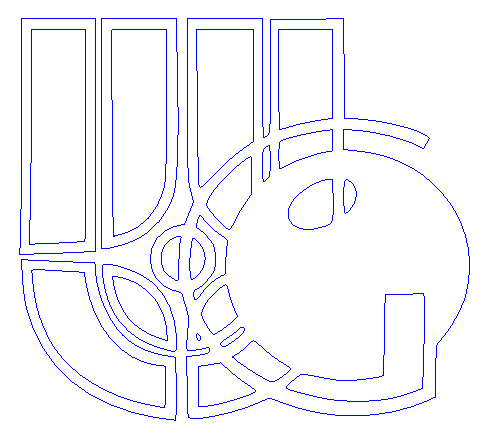
\includegraphics[height=65pt]{logos/logo_kipnpi.eps}}

    % QR-код ОПР (слева).
    \put(0.42,1.05){\color{white}\qrcode[hyperlink,height=.09\textwidth]{https://www.pnpi.nrcki.ru/}}
    %\put(0.59,0.0){\small\bf\color{white}ОПР ПИЯФ}

    \end{picture}
}
{
    % Авторы (уже указаны в заголовке)
}
{
    % Логотип (уже вставлен в заголовок)
}

% ==================== НИЖНИЙ КОЛОНТИТУЛ ====================
\headerbox{}{name=foottext, column=0, span=6,
    above=bottom, headershape=rectangle,
    textborder=none, borderColor=NSMD, boxheaderheight=0pt, boxpadding=0.5em}{%               
    \hspace*{-1.8em}
    \begin{minipage}[t]{0.10\textwidth}
        \FooterContactSize
        \textbf{Троцай Н.А.}\\
        % ОНСМ ОПР\\
        % НИЦ «КИ»~--- ПИЯФ\\
        nikitatrotsay@gmail.com
        \vspace{-0.2cm}\\
        \qrcode[height=1.5cm]{mailto:nikitatrotsay@gmail.com}%
    \end{minipage}%
    \hfill
    \vrule
    \hfill
    \begin{minipage}[t]{0.8\textwidth}
        \textbf{\FooterBibHeadSize\color{NSMD}ОСНОВНЫЕ ИСТОЧНИКИ}
        \vspace{0.02cm}%
        \FooterBibSize
        \setlength{\bibitemsep}{0pt}%
        \setlength{\bibparsep}{0pt}%
        \printbibliography[heading=none]
    \end{minipage}%
}

% ==================== ОСНОВНЫЕ БЛОКИ ПОСТЕРА ====================

% БЛОК 1: Введение
\headerbox{Введение}{name=introduction, column=0, row=0, span=3}
{%
    \BoxBodySize
    \emph{Нейтронно-активационный анализ} --- один из наиболее чувствительных методов определения элементного состава вещества. В основе метода лежит принцип регистрации гамма-квантов от радионуклидов, образующихся при захвате нейтронов. Метод имеет ряд достоинств: широкий диапазон регистрируемых элементов, низкие пределы их обнаружения, отсутствие влияния химического состояния элемента, малые навески образца.

    В НИЦ «Курчатовский институт»~--- ПИЯФ в рамках подготовки программы фундаментальных и прикладных исследований на реакторе ПИК проводятся методические работы по нейтронно-активационному анализу; для их осуществления создана установка СТЕНА (СТЕнд Нейтронной Активации). Установка дает возможность проведения мгновенного и задержанного инструментального \linebreak нейтронно-активационного анализа (НАА).
}

% БЛОК 2: Установка
\headerbox{Экспериментальный стенд}{name=vmeas, span=3, below=introduction, column=0}{%
    \BoxBodySize
    \noindent
    \begin{minipage}[t]{0.48\textwidth}
        \vspace{0pt}%  
        \emph{Источник нейтронов ИБН-8-5}~\cite{mayak2020} с активностью $2\text{,}4\cdot{10}^{11}$\,Бк (на момент изготовления) обеспечивает полный нейтронный поток $0\text{,}95(20)\cdot{10}^7$~с$^{-1}$. Спектр нейтронов от источника ИБН-8-5 простирается до энергии $10$\,МэВ при средней энергии $\approx 4{,}5$\,МэВ. Спектрометрический тракт состоит из коаксиального детектора на основе HPGe, предусилителя и анализатора.
        Конструкция радиационной защиты установки разработана с учётом модельных спектров излучения $\mathrm{Pu-Be}$-источника (рис.~\ref{fig:neutron} и рис.~\ref{fig:gamma})~\cite{ershov2018}. 
        Срок службы источника, представляющего собой цилиндр диаметром
        18\,мм и высотой 22\,мм, ограничен коррозионной стойкостью его корпуса и составляет~10\,лет.
        \vspace{0.5em}
    \end{minipage}\hfill
    \begin{minipage}[t]{0.48\textwidth}
        \vspace{0pt}%  % включает выравнивание [t] по верхнему краю
        \centering
        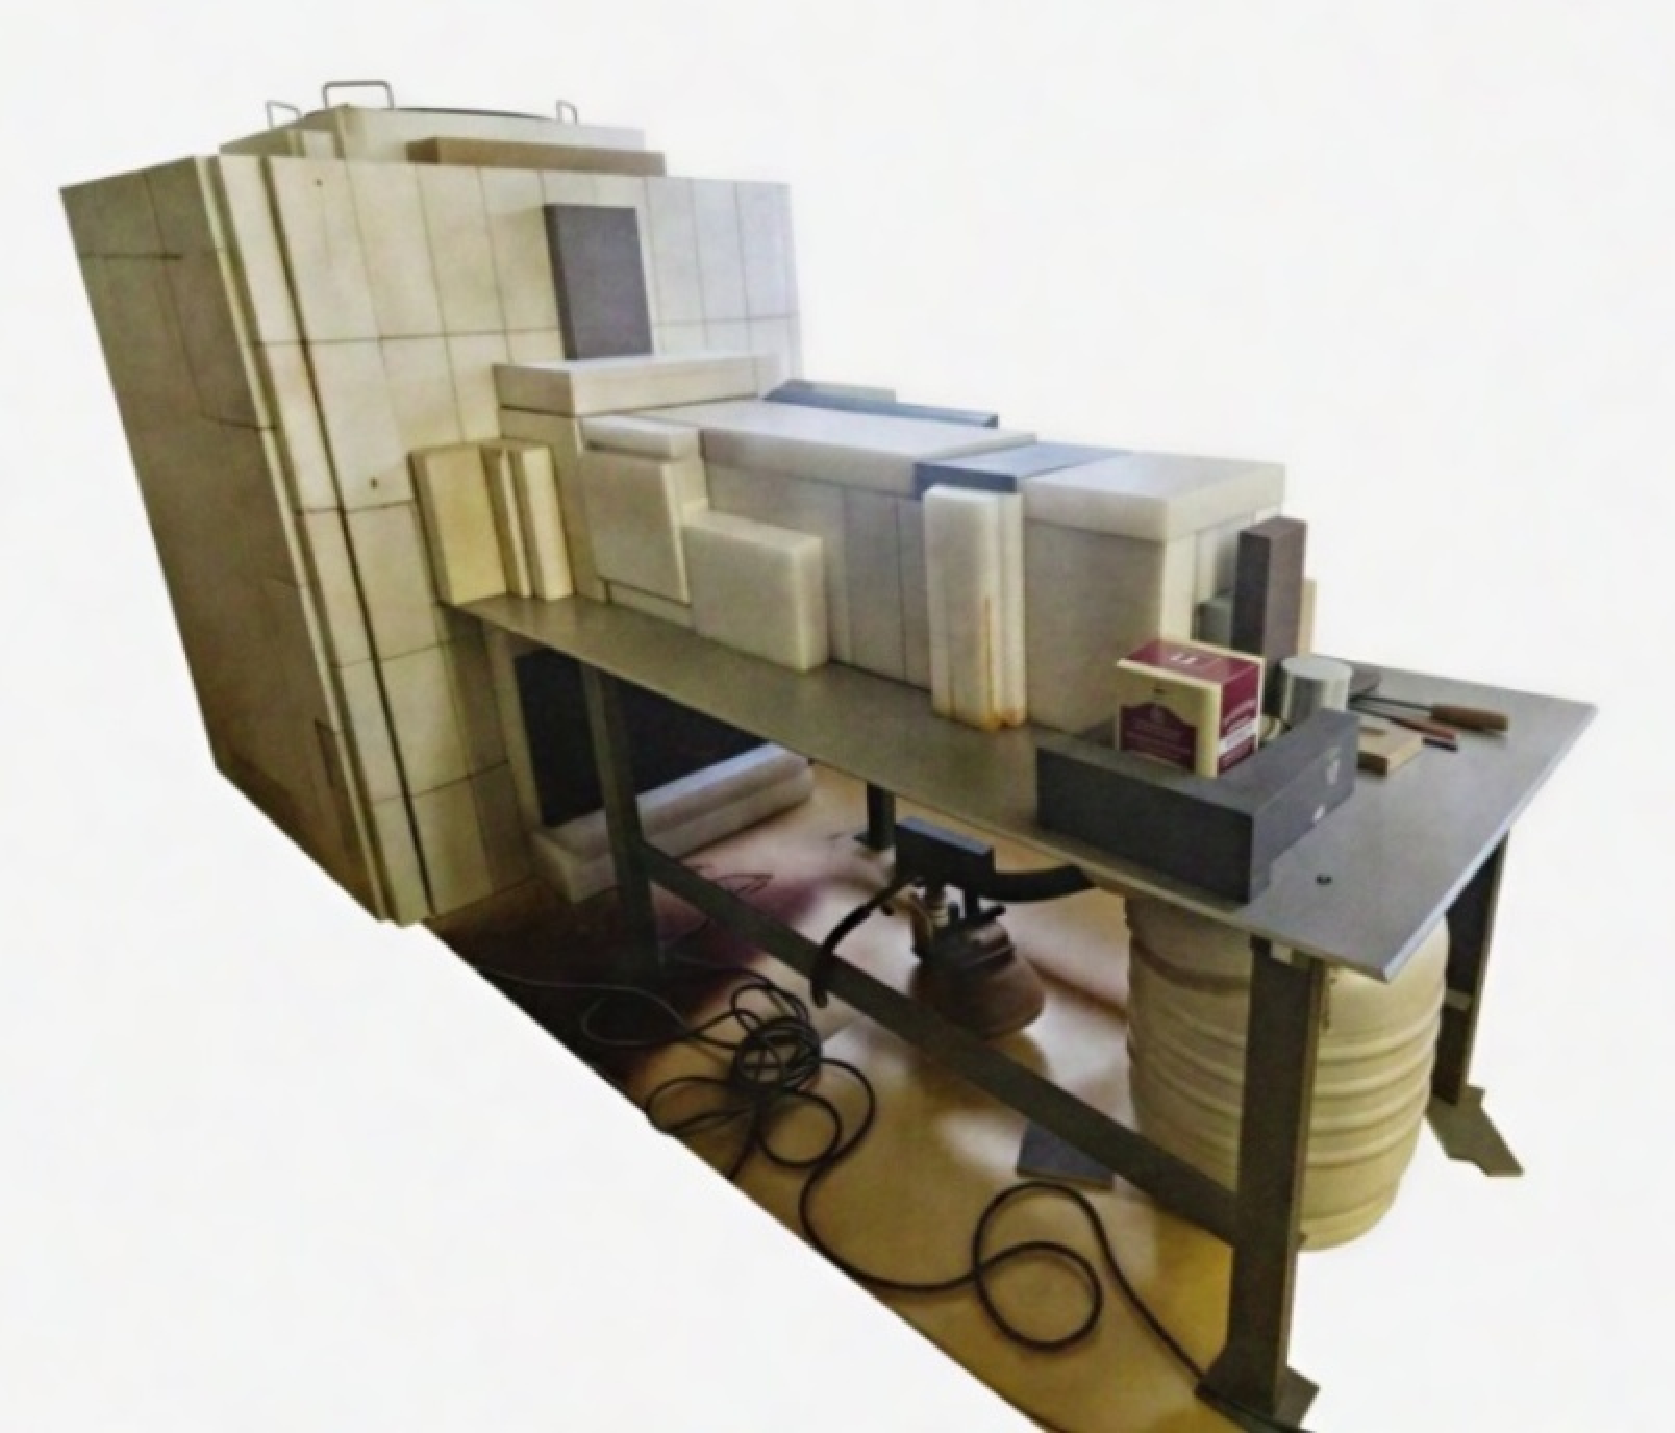
\includegraphics[width=0.9\textwidth, keepaspectratio]{Images/setup.pdf}
        \captionof{figure}{Общий вид установки нейтронного облучения СТЕНА}
        \label{fig:setup}
    \end{minipage}
    \vspace{-0.3cm}
    \begin{center}
        % Левый график — нейтроны
        \begin{minipage}[t]{0.48\textwidth}
            \centering
            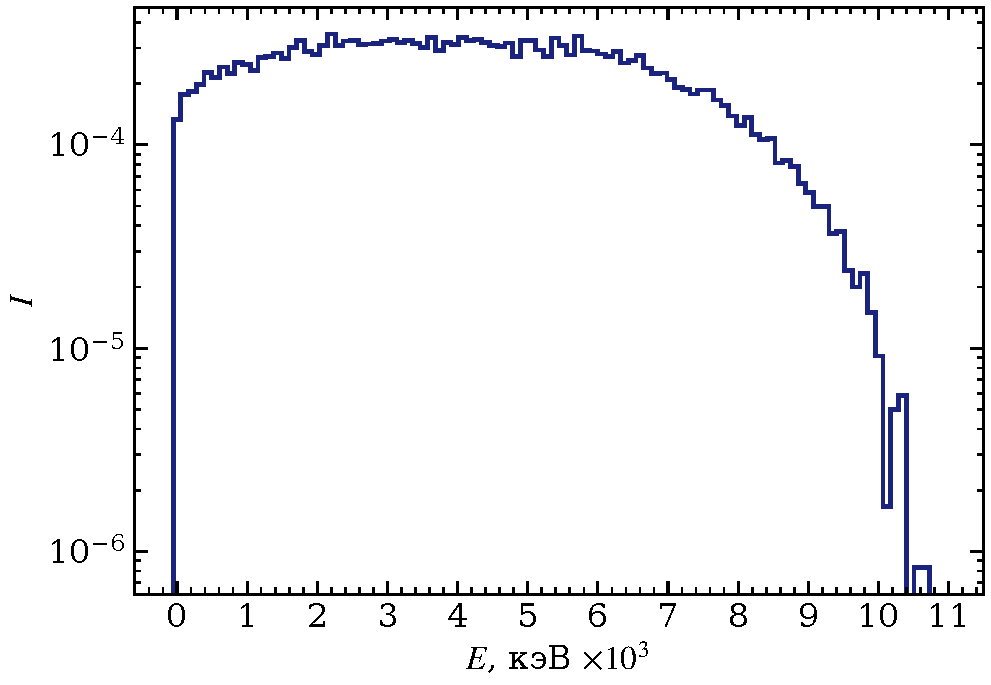
\includegraphics[width=\linewidth, keepaspectratio]{Images/neutron_spectrum_stairs.pdf}
            \captionof{figure}{Расчетный спектр нейтронного излучения Pu--Be-источника}
            \label{fig:neutron}
        \end{minipage}\hfill
        % Правый график — гамма
        \begin{minipage}[t]{0.48\textwidth}
            \centering
            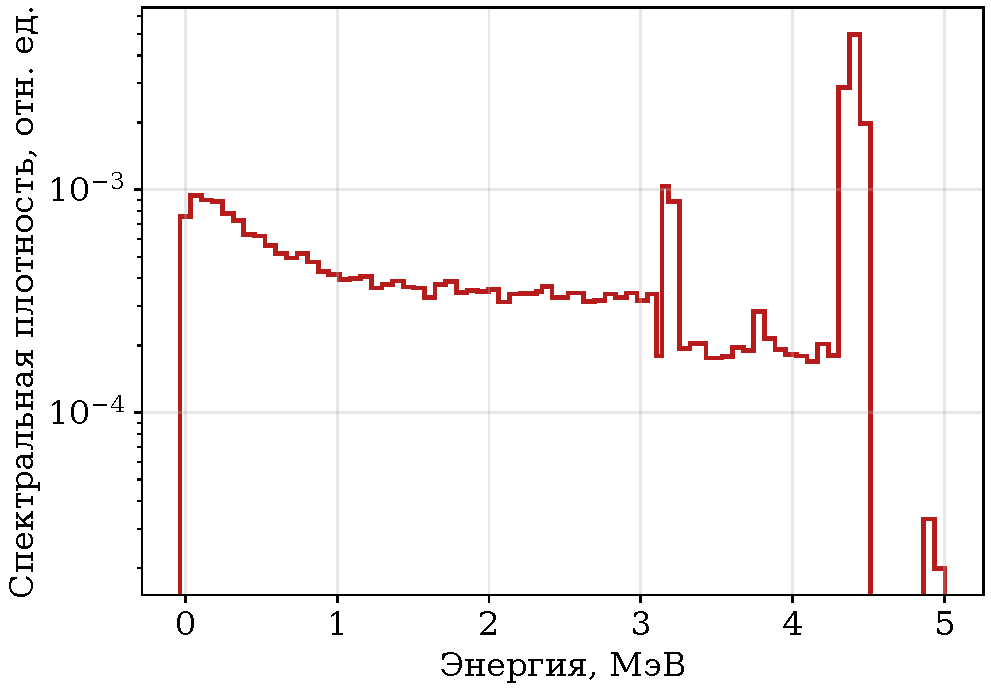
\includegraphics[width=\linewidth, keepaspectratio]{Images/gamma_spectrum_stairs.pdf}
            \captionof{figure}{Расчетный спектр гамма-излучения Pu--Be-источника}
            \label{fig:gamma}
        \end{minipage}
    \end{center}
}

\headerbox{Калибровка эффективности}{name=summary, span=3, below=vmeas, column=0}{%
    \BoxBodySize
    % ==================== ВЕРХНИЙ РЯД: текст + 1-й график ====================
    \noindent
    \begin{minipage}[t]{0.48\textwidth}
        \vspace{0pt}%
        Для построения калибровочных зависимостей эффективности регистрации гамма-излучения использовались точечный и плоский источники на основе смеси изотопов $^{133}\mathrm{Ba}$ и $^{201}\mathrm{Bi}$ c равной активностью. Зависимости аппроксимировались функцией вида:
        \vspace{-0.5em}
        \begin{equation}
            \varepsilon(E)\!=\!\varepsilon_0 \, E^{-\alpha}
            \bigl[ 1\!+\!e^{-(E\!-\!E_{\mathrm{th}})/\Delta E} \bigr]^{-1},
            \label{eq:eff}
        \end{equation}
        где \(\varepsilon_0\) --- параметр нормировки;\\
        \(\alpha\) --- эффективный показатель спада;\\ 
        \(E_{\text{th}}\) --- порог регистрации, кэВ;\\
        \(\Delta E\) --- ширина порога регистрации, кэВ.
    \end{minipage}\hfill
    \begin{minipage}[t]{0.48\textwidth}
        \vspace{0pt}%
        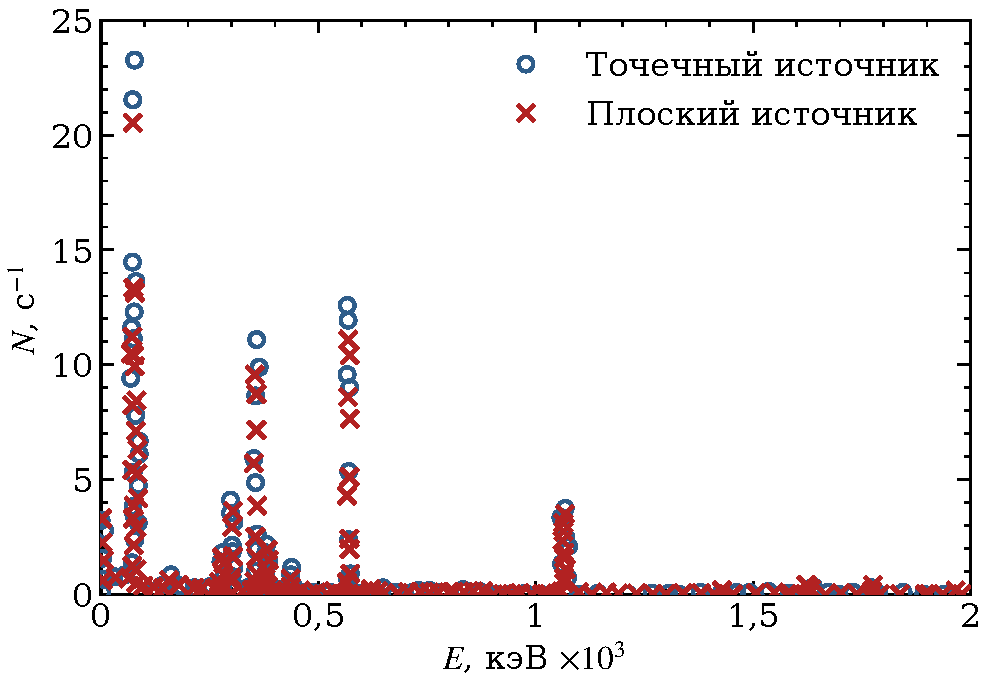
\includegraphics[width=\linewidth, keepaspectratio]{Images/gamma_spectra_points.pdf}
        \captionof{figure}{Спектры гамма-излучения точечного (синие точки) и плоского (красные крестики) стандартных источников}
        \label{fig:spectra-eff}
    \end{minipage}

    % ==================== НИЖНИЙ РЯД: 2-й график + 3-й график ====================
    \vspace{0.3em}
    \noindent
    \begin{minipage}[t]{0.48\textwidth}
        \vspace{0pt}%
        \centering
        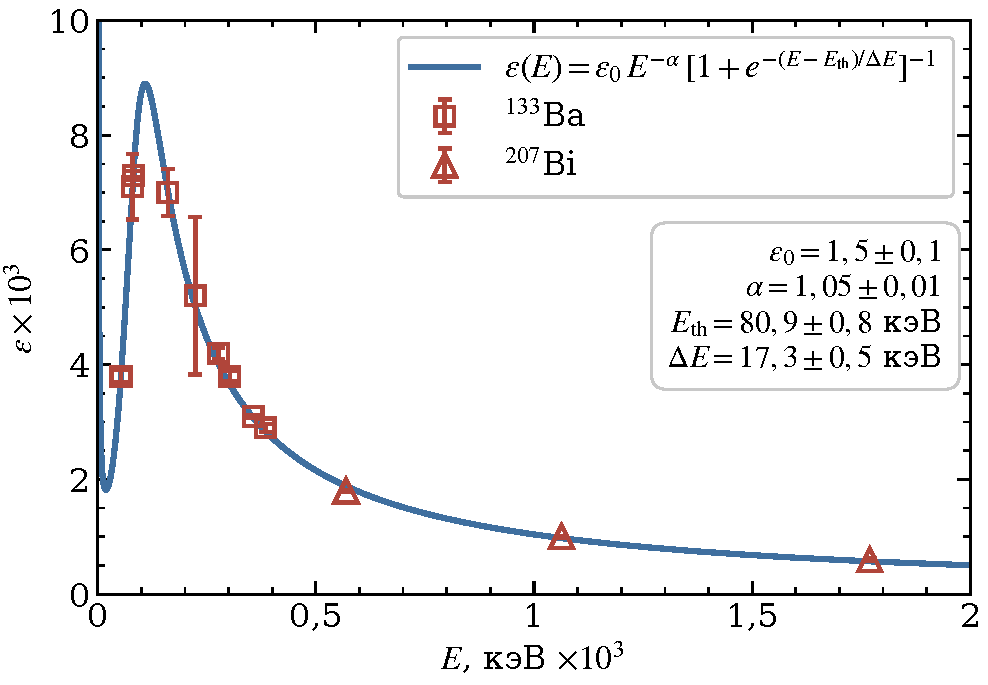
\includegraphics[width=\linewidth, keepaspectratio]{Images/efficiency_calibration.pdf}
        \captionof{figure}{Калибровочная зависимость эффективности регистрации гамма-излучения для точечного источника}
        \label{fig:gamma-caliber}
    \end{minipage}\hfill
    \begin{minipage}[t]{0.48\textwidth}
        \vspace{0pt}%
        \centering
        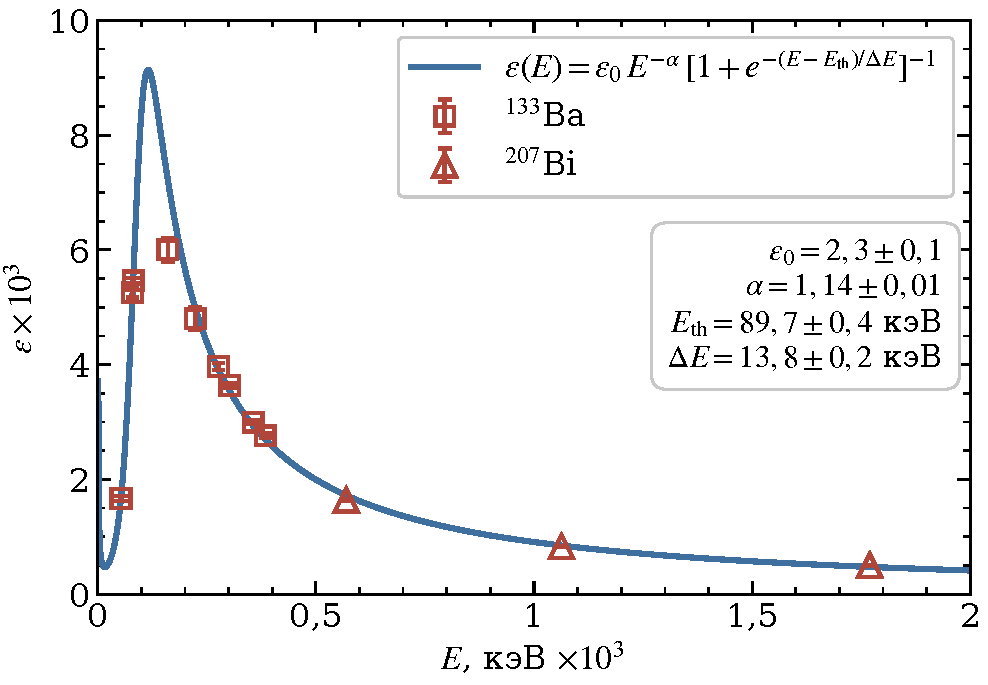
\includegraphics[width=\linewidth, keepaspectratio]{Images/efficiency_calibration_flat.pdf}
        \captionof{figure}{Калибровочная зависимость эффективности регистрации гамма-излучения для плоского источника}
        \label{fig:gamma_caliber_flat}
    \end{minipage}
}

% БЛОК 4: Детали / Данные (правая колонка, самый верх)
\headerbox{Активация брома}{name=resolution, span=3, row=0, column=3}{%
    \BoxBodySize
    % ==================== ВЕРХНИЙ РЯД: текст + 1-й график ====================
    \noindent
    \begin{minipage}[t]{0.48\textwidth}
        \vspace{0pt}%
        \noindent
        Первый опыт по нейтронной активации проведён с образцом бромида калия, размещённым внутри водяной полости. Естественная смесь изотопов брома. В результате активации образуются четыре долгоживущих состояния брома. Гамма-спектры активированного образца измерялись офлайн четыре раза сеансами разной длительности. По измеренным данным построена распадная зависимость и вычислено значение периода полураспада $^{82}\mathrm{Br}$ $T_{1/2}=1{,}45(3)$~сут, согласующееся с табличным $1{,}4701(3)$~сут~\cite{iaea_livechart} в пределах погрешности.
    \end{minipage}\hfill
    \begin{minipage}[t]{0.48\textwidth}
        \vspace{0pt}%
        \centering
        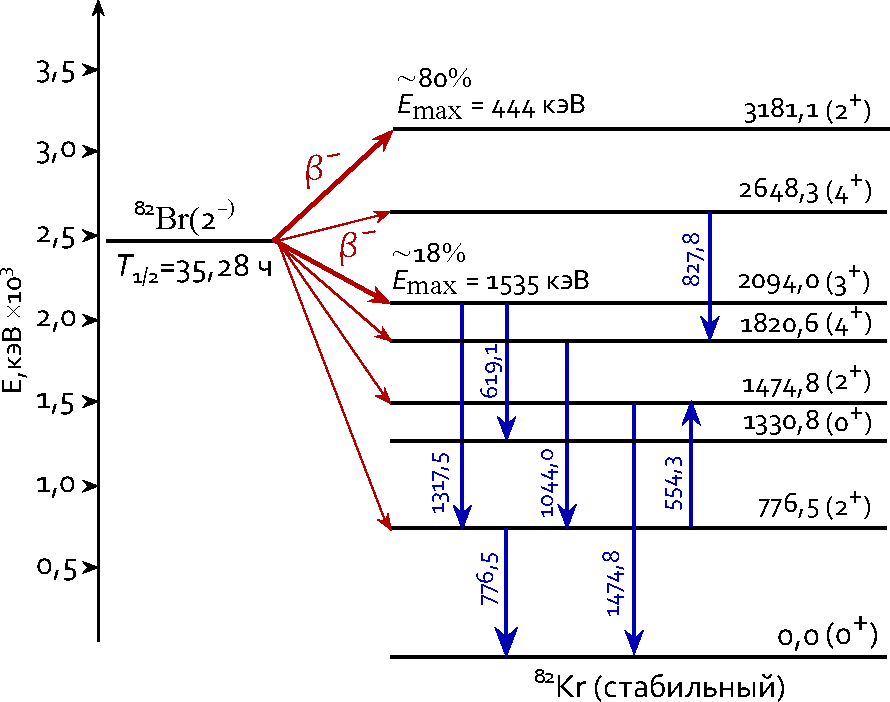
\includegraphics[width=\linewidth, keepaspectratio]{Images/82B_decay.pdf}
        \captionof{figure}{Сокращенная схема распада $^{82}\mathrm{Br}$}
        \label{fig:decay-br-scheme}
    \end{minipage}


    % ==================== НИЖНИЙ РЯД: 2-й график ====================
    \vspace{0.3em}
    \noindent
        \begin{minipage}[t]{0.48\textwidth}
        \vspace{0pt}%
        \centering
        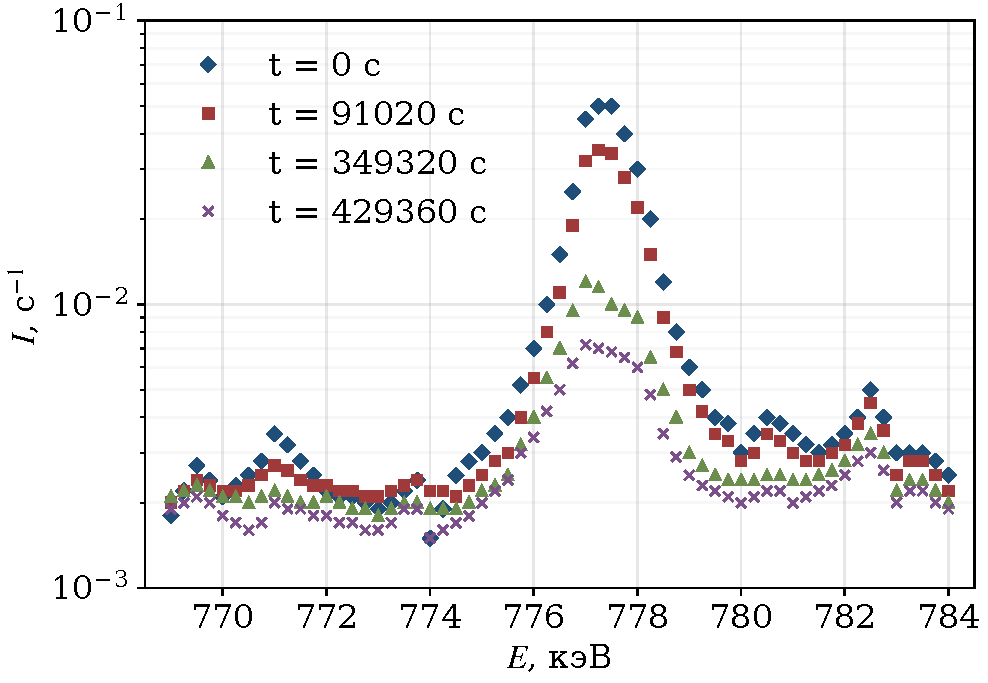
\includegraphics[width=\linewidth, keepaspectratio]{Images/spectra_points.pdf}
        \captionof{figure}{Задержанные на время распада $t$ спектры гамма-излучения в распаде  $^{82}\mathrm{Br}$}
        \label{fig:spectra-br}
    \end{minipage}\hfill
        \begin{minipage}[t]{0.48\textwidth}
        \vspace{0pt}%
        \centering
        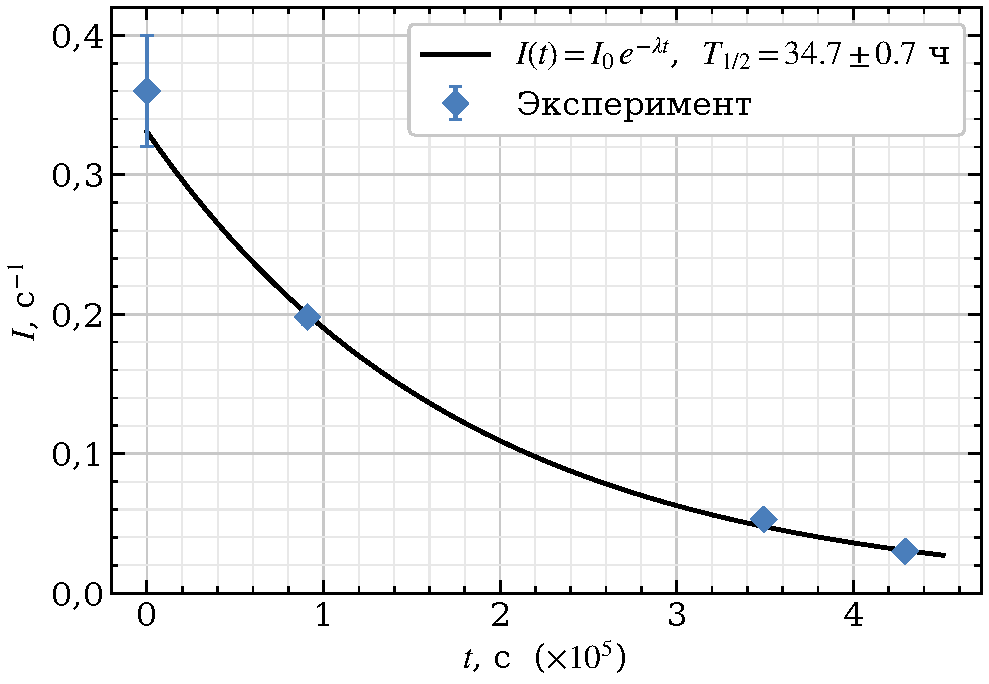
\includegraphics[width=\linewidth, keepaspectratio]{Images/decay_fit.pdf}
        \captionof{figure}{Кривая распада  $^{82}\mathrm{Br}$}
        \label{fig:decay-br-curve}
    \end{minipage}\hfill

}


\headerbox{Активация золота}{name=motivation, below=resolution, span=3, row=0, column=3}{%
    \BoxBodySize
    % ==================== ВЕРХНИЙ РЯД: текст ====================
    \noindent
    \begin{minipage}[t]{0.96\textwidth}
        Аналогичным методом проведена активация золота; в качестве образца использована навеска единственного природного изотопа $^{197}\mathrm{Au}$ массой $28\text{,}5$\,мг, воздействие производилось тепловыми и эпитепловыми нейтронами. В первом опыте образец облучался полным потоком нейтронов от источника, после чего по гамма-линии $411\text{,}8$\,кэВ измерялся период полураспада $^{198}\mathrm{Au}$. Во втором опыте для выделения эпитепловой компоненты использовался кадмиевый фильтр, поглощающий тепловые нейтроны. По измеренным активностям для исследованного образца определены плотности потоков эпитепловых нейтронов.
        \vspace{0.5em}
    \end{minipage}
    % % ==================== НИЖНИЙ РЯД: 2-й график ====================
    \noindent
    \begin{minipage}[t]{0.48\textwidth}
        \vspace{0pt}%
        \centering
        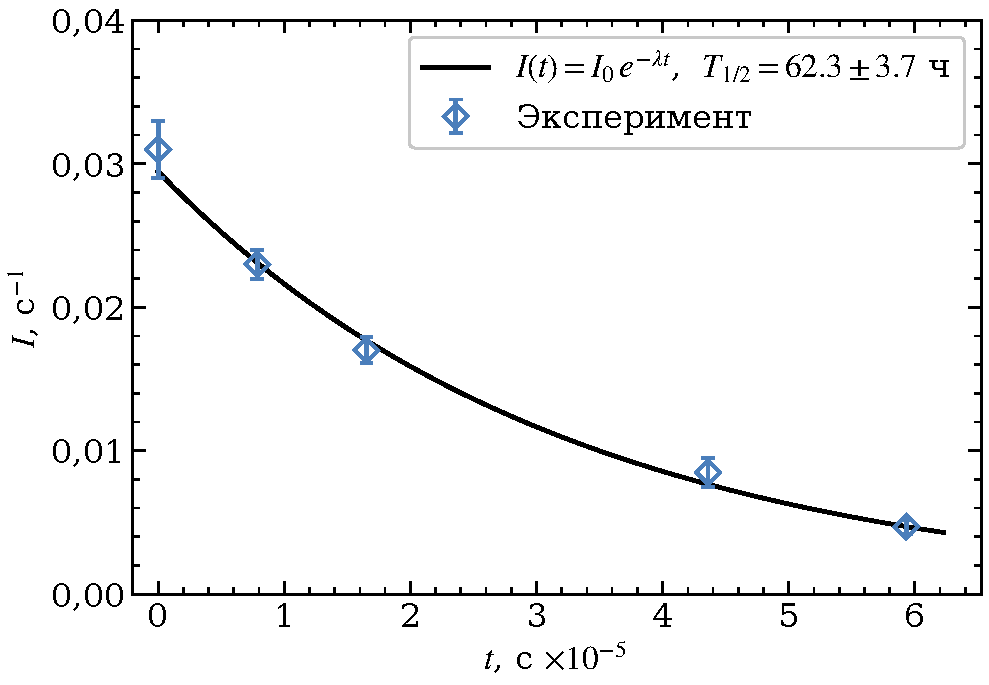
\includegraphics[width=\linewidth, keepaspectratio]{Images/decay_fit_2.pdf}
        \captionof{figure}{Кривая распада $^{198}\mathrm{Au}$}
        \label{fig:spectra-Au}
    \end{minipage}\hfill
    \begin{minipage}[t]{0.48\textwidth}
        \vspace{0pt}%
        \centering
        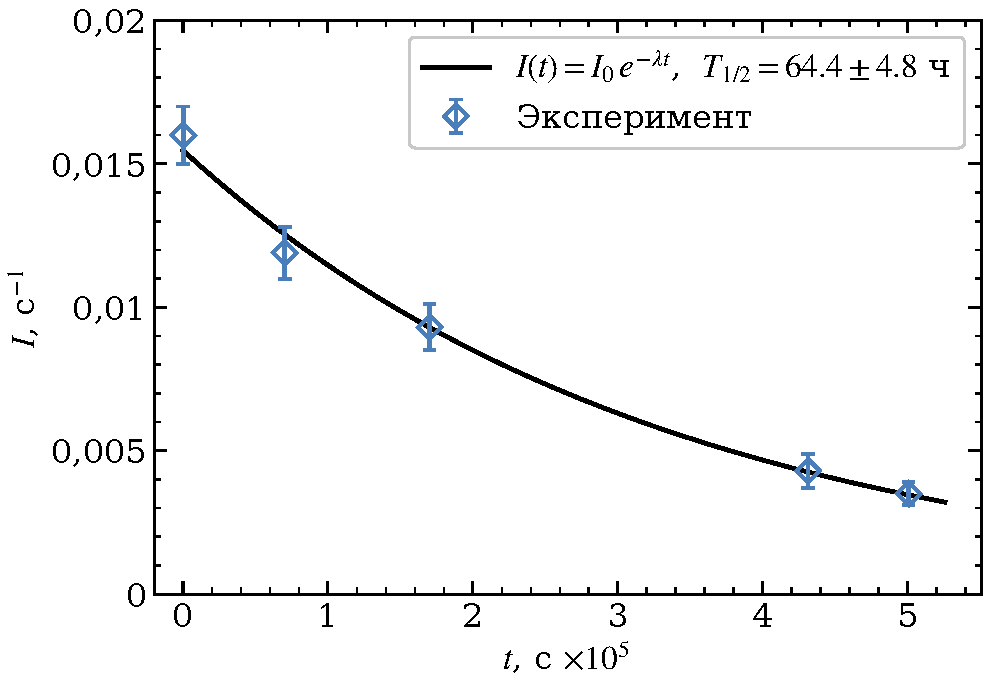
\includegraphics[width=\linewidth, keepaspectratio]{Images/decay_fit_new.pdf}
        \captionof{figure}{Кривая распада $^{198}\mathrm{Au}$ (облучение с кадмиевым фильтром)}
        \label{fig:spectra-Au-2}
    \end{minipage}
}

\headerbox{Перспективы: анализ эндофуллеренов}{name=endo, below=motivation, span=3, row=0, column=3}{%
    \BoxBodySize
    % ==================== ТЕКСТ ====================
    \noindent
    \begin{minipage}[t]{0.96\textwidth}
        Здесь будет краткое описание задачи по анализу эндофуллеренов:
        методика облучения образцов, регистрация гамма-спектров,
        обработка данных. Текст-заглушка для оценки вёрстки
        (примерно 5--7 строк), чтобы блок занял нужную высоту
        и не «схлопнулся» при компиляции без рисунка.
        \vspace{0.5em}
    \end{minipage}

    % ==================== РИСУНОК ВНИЗУ (на всю ширину) ====================
    \noindent
    \begin{minipage}[t]{0.96\textwidth}
        \vspace{0pt}%
        \centering
        % --- ЗАГЛУШКА: пустая рамка нужного размера ---
        \fbox{\begin{minipage}[c][5cm][c]{0.98\linewidth}
            \centering\color{gray}\small
            [ Место для рисунка ]\\
            (заменить на \texttt{\textbackslash includegraphics})
        \end{minipage}}
        \captionof{figure}{Подпись к рисунку (заглушка)}
        \label{fig:endo}
    \end{minipage}
}

% ==================== КОНЕЦ ПОСТЕРА ====================
\end{poster}
\end{document}